\documentclass[11pt]{article}
\usepackage[margin=1in]{geometry}
\usepackage{titlesec}
\usepackage{url}
\usepackage{hyperref}
\usepackage{amsmath}
\usepackage{amssymb}
\usepackage{enumitem} % in preamble
\usepackage{graphicx}
\usepackage{pgfplots}
\usepackage{booktabs}
\usepackage{siunitx}
\pgfplotsset{compat=1.18}

\sisetup{
  group-digits=false,
  round-mode=places,
  round-precision=6
}
\graphicspath{{../Screenshots/}}
\setlist[itemize]{leftmargin=*, nosep, topsep=0pt, partopsep=0pt}

\newcommand{\memoheader}[4]{
  \noindent
  \textbf{From:} #2\\ 
  \textbf{To:} #1\\
  \textbf{Date:} #3\\
  \textbf{Subject:} #4\\[1ex]\hrule\vspace{1.5ex}
}

\begin{document}
\memoheader{Prof. Susan Gentry}
            {Miguel Cuaycong}
            {\today}
            {EMS 164: HW 1}
\section{Porter and Easterling 2.2}
-INTENTIONALLY BLANK. Didnt have time to solve this one
\section{Proof by differentiation}
Governing equation: $c_i(x,t) = \frac{N_i}{\sqrt{4 \pi Dt}}e^{-\frac{x^2}{4Dt}}$
\\~\\
We are trying to prove: $\frac{dc_i}{dt} = D_i\frac{d^2C_i}{dx^2}$
\\~\\
For $\frac{d}{dt}c_i(x,t)$:
\begin{align*}
  \frac{d}{dt}c_i(x,t) &= \frac{d}{dt}(\frac{N_i}{\sqrt{4 \pi Dt}}e^{-\frac{x^2}{4Dt}})
  \\
  \frac{dc_i(x,t)}{dt} &= \frac{d}{dt}(\frac{N_i}{\sqrt{4 \pi Dt}})(e^{-\frac{x^2}{4Dt}}) + \frac{N_i}{\sqrt{4 \pi Dt}}\frac{d}{dt}(e^{-\frac{x^2}{4Dt}})
  \\
  \frac{dc_i(x,t)}{dt} &= -\frac{1}{2}(\frac{N_i}{\sqrt{4 \pi Dt^3}})(e^{-\frac{x^2}{4Dt}}) + \frac{N_i}{\sqrt{4 \pi Dt}}\frac{x^2}{4Dt^2}(e^{-\frac{x^2}{4Dt}})
  \\
  \frac{dc_i}{dt} &= (-\frac{1}{2t}+\frac{x^2}{4Dt^2})(e^{-\frac{x^2}{4Dt}})(\frac{N_i}{\sqrt{4 \pi Dt}}) 
  \\
  \end{align*}
  $\text{ let } A = \frac{N_i}{\sqrt{4 \pi Dt}},  \text{ and } B_t = (e^{-\frac{x^2}{4Dt}})$: 
  $$\frac{dc_i}{dt} = (-\frac{1}{2t}+\frac{x^2}{4Dt^2})B_tA$$
  \\

For $\frac{d^2C_i}{dx^2}$:
\begin{align*}
  \frac{d^2c_i}{dx^2} &= \frac{d^2}{dx^2}(\frac{N_i}{\sqrt{4 \pi Dt}}e^{-\frac{x^2}{4Dt}})
  \\
  \frac{d^2c_i}{dx^2} &= A\frac{d^2}{dx^2}(e^{-\frac{x^2}{4Dt}}) = A\frac{d}{dx}(e^{-\frac{x^2}{4Dt}}(-\frac{x}{2Dt}))
  \\
  \frac{d^2c_i}{dx^2} &= A(e^{-\frac{x^2}{4Dt}}(-\frac{x}{2Dt})^2+e^{-\frac{x^2}{4Dt}}(-\frac{1}{2Dt}))
  \\
  \frac{d^2c_i}{dx^2} &= AB_t(-\frac{1}{2t}+\frac{x^2}{4Dt})\frac{1}{D}
\end{align*}
Now we can prove $\frac{dc_i}{dt} = D_i\frac{d^2C_i}{dx^2}$:
\begin{align*}
  \frac{dc_i}{dt} = D_i\frac{d^2C_i}{dx^2} &\rightarrow (-\frac{1}{2t}+\frac{x^2}{4Dt^2})AB_t = D\frac{1}{D}(-\frac{1}{2t}+\frac{x^2}{4Dt})AB_t
  \\
  &\rightarrow (-\frac{1}{2t}+\frac{x^2}{4Dt^2})AB_t = (-\frac{1}{2t}+\frac{x^2}{4Dt})AB_t
  \\
  &\mathbf{\therefore \frac{dc_i}{dt} = D_i\frac{d^2C_i}{dx^2}}
\end{align*}
\section{The reaction rate of a thermally-activated corrosion process }
The calculations are done on Desmos.

% ---------- Table with 1/T and ln(k) ----------
\begin{table}[h]
\centering
\caption{Arrhenius-transform values (T in Kelvin).}
\begin{tabular}{S[table-format=4.2] S[scientific-notation=true] S[table-format=-2.6]}
\toprule
{$T$ (K)} & {$1/T$ (K$^{-1}$)} & {$\ln(k)$} \\
\midrule
1573.15 & 6.35668e-4 & -12.311433 \\
1673.15 & 5.97676e-4 & -10.829829 \\
1723.15 & 5.80333e-4 &  -9.841452 \\
1773.15 & 5.63968e-4 &  -9.323509 \\
1873.15 & 5.33860e-4 &  -8.468403 \\
\bottomrule
\end{tabular}
\end{table}

% ---------- Arrhenius plot: ln(k) vs 1/T ----------
\begin{figure}[h]
\centering
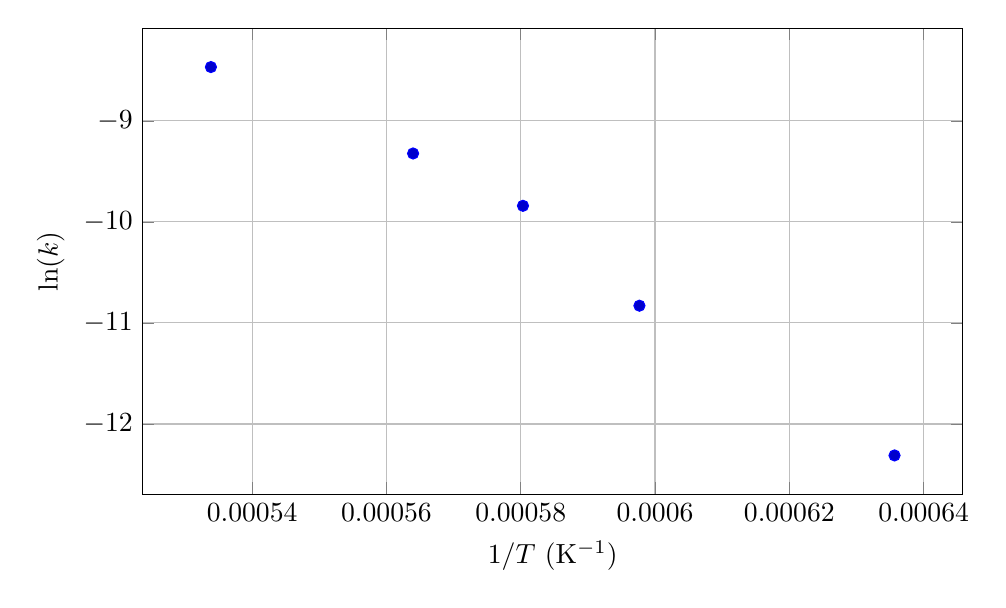
\begin{tikzpicture}
\begin{axis}[
  width=12cm,
  height=7.5cm,
  grid=both,
  xlabel={$1/T\ (\mathrm{K}^{-1})$},
  ylabel={$\ln(k)$},
  scaled x ticks=false, % show full decimal ticks (no \times 10^{...})
  x tick label style={
    /pgf/number format/fixed,
    /pgf/number format/precision=7
  }
]
\addplot+[
  only marks,
  mark=*,
] table[row sep=\\, x=invT, y=lnk]{
invT        lnk\\
0.000635668 -12.311433\\
0.000597676 -10.829829\\
0.000580333  -9.841452\\
0.000563968  -9.323509\\
0.000533860  -8.468403\\
};
\end{axis}
\end{tikzpicture}
\caption{Arrhenius plot of the corrosion-rate data (\(\ln(k)\) vs \(1/T\), with \(T\) in K).}
\end{figure}

Linear fit equation: $m = -38645.63, b = 12.348$
\\~\\
To calculate activation energy, use: $m = -\frac{\Delta G_{act}}{R} \rightarrow \Delta G_{act} = -mR = 38645.63*8.314 [K\frac{J}{molK}] = \mathbf{321kJ/mol}$
\section{Research laboratory that operates a furnace filled with helium to
maintain an inert environment}
The most appropriate model is (I think) Steady-state diffusion through plate from lecture:
\begin{center}
  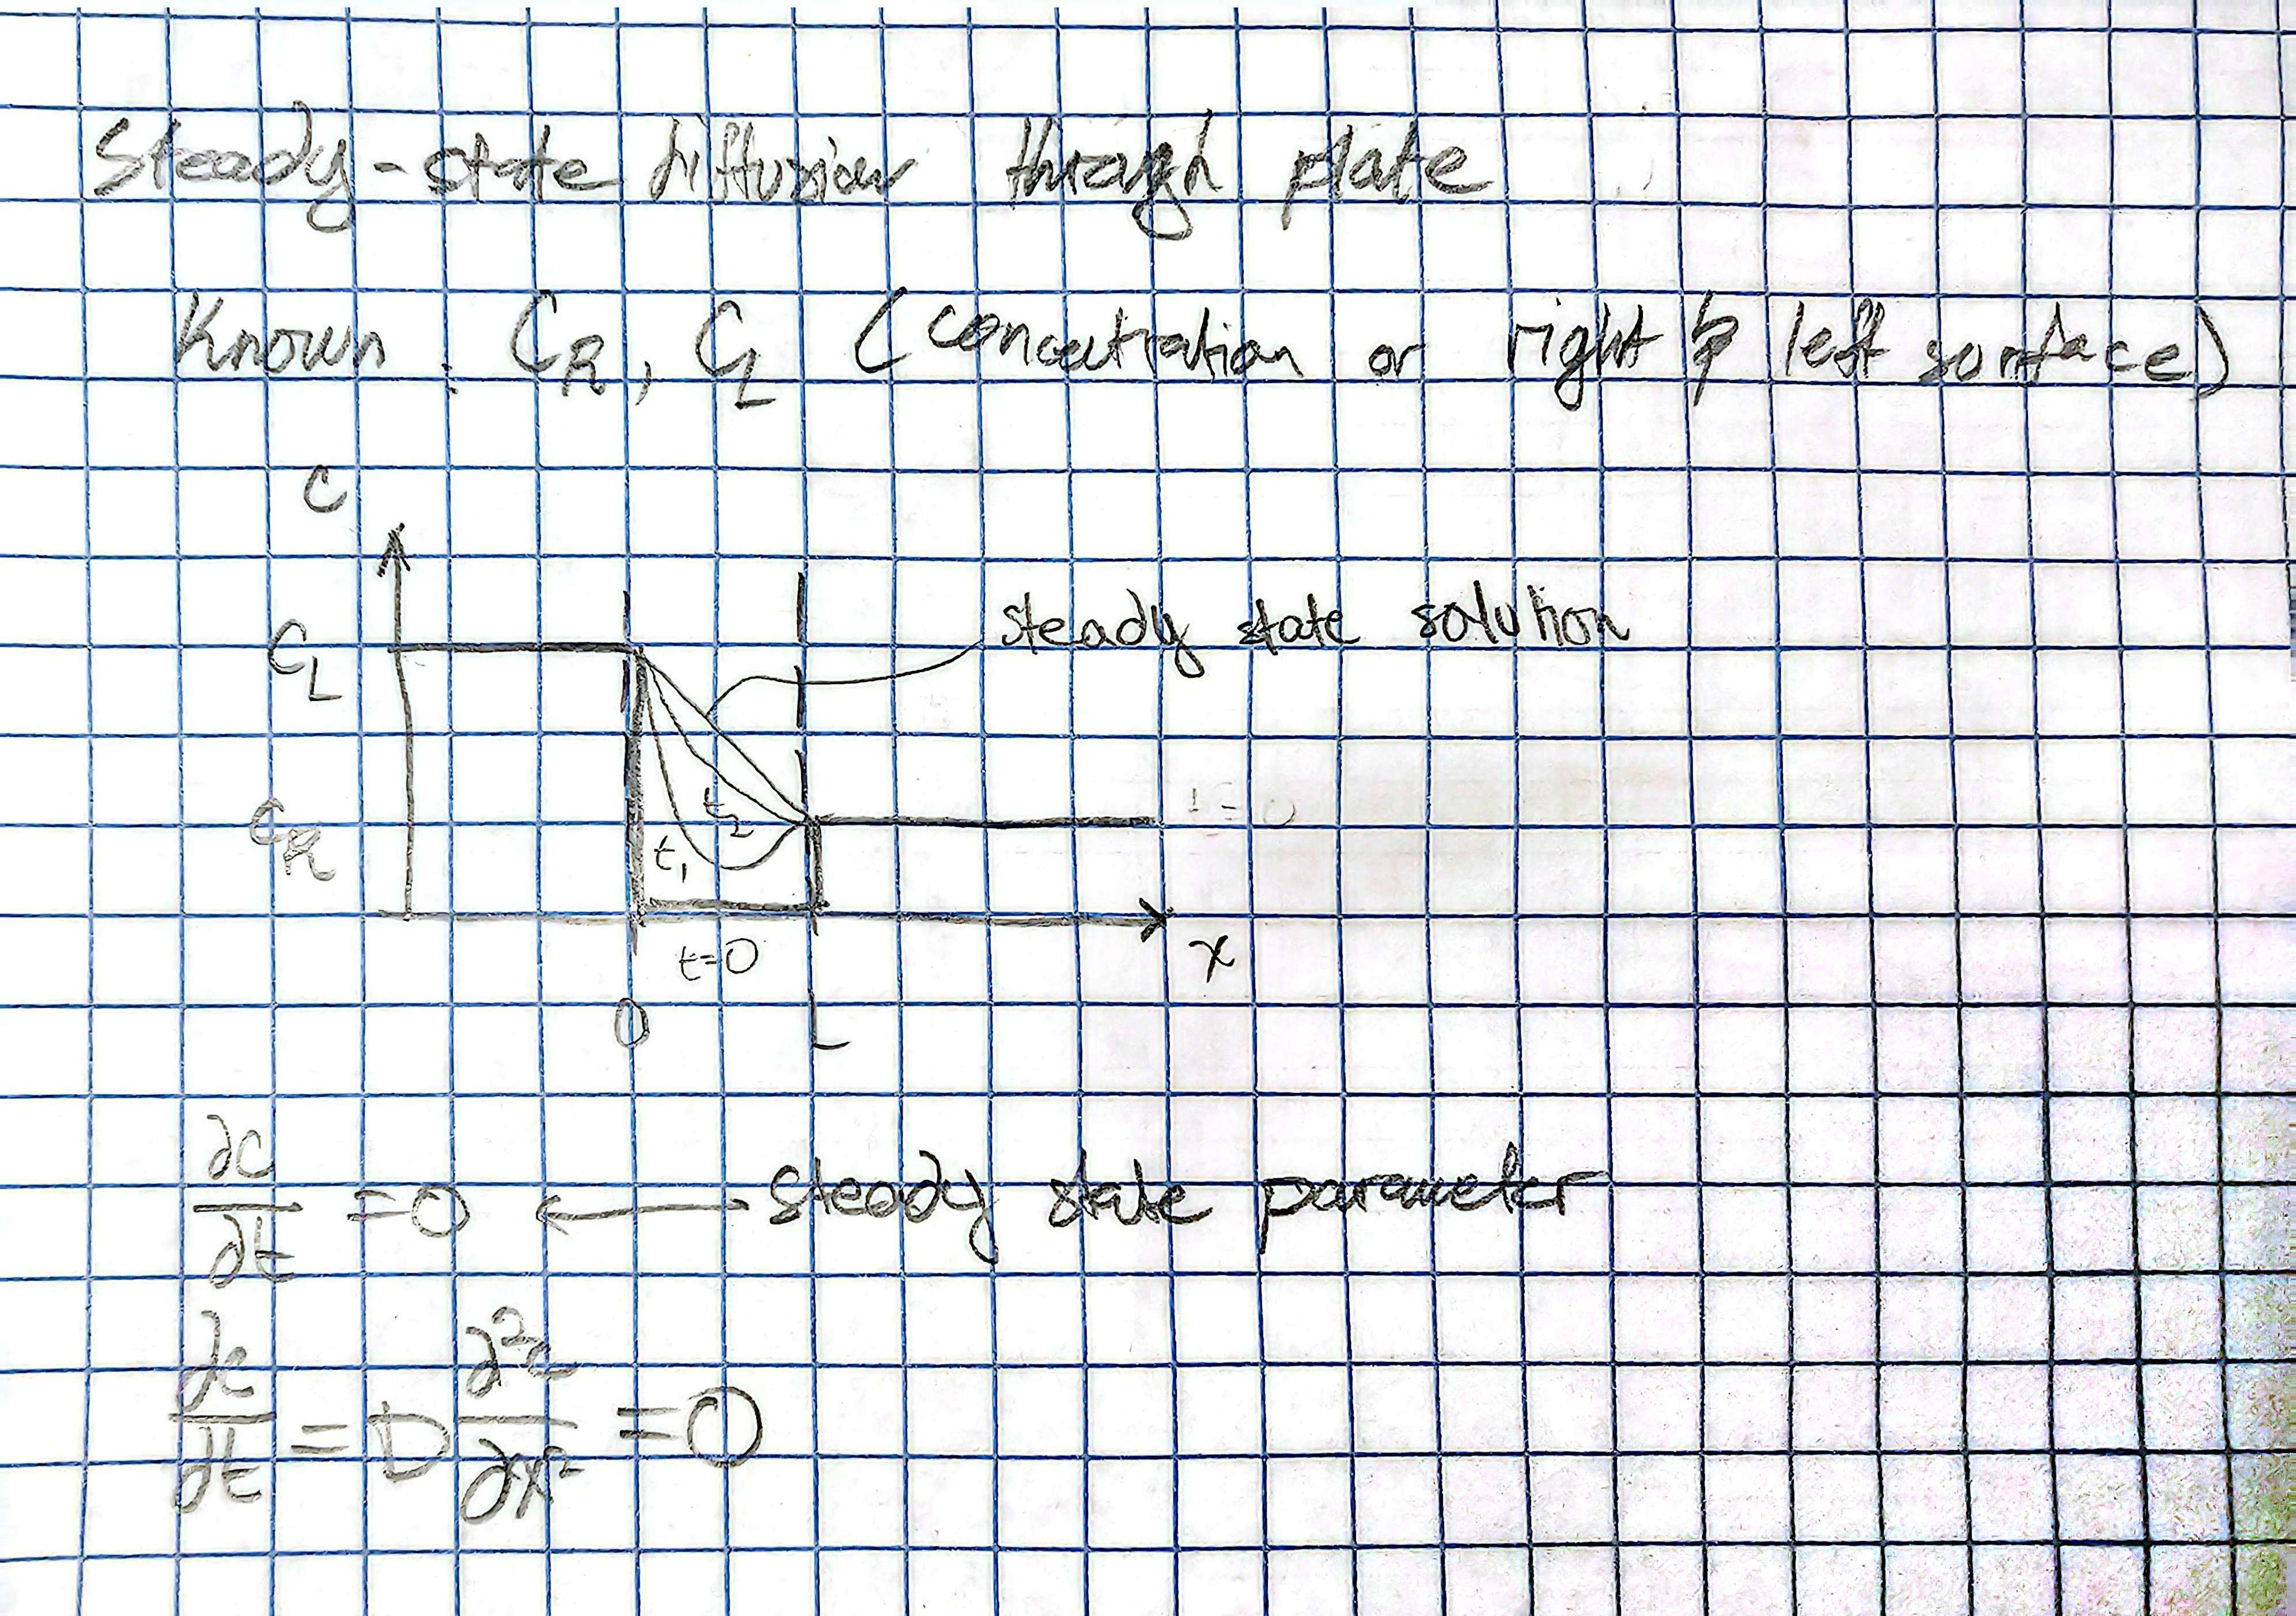
\includegraphics[width=250pt]{ssdiffusion.jpg}
\end{center}
\begin{align*}
  &c(x=0, t=\infty)=c_L
  \\
  &c(x=L, t=\infty)=c_R = 0 \rightarrow\text{This assumes the right side is the outside with no helium}
\end{align*}
Deduce the concentration term for ideal gas law: $PV = nRT = N\frac{R}{N_A}T$ where N is atoms and $N_A$ is avogadro's number.
$N/V=\frac{PN_A}{RT} \rightarrow c = \frac{PN_A}{RT}$
\\
$c_L$ can now be calculated: $c_L = \frac{(10)(1.01325(10)^5)(6.022(10)^{23})}{8.314(1273.15)} = 5.77(10)^{25}\text{ atoms}/m^3$ 
\\
solution was derived in class as: $c = \frac{c_R-c_L}{L}x+c_L$
\\
ANSWER: steady state flux is: $J = -D\frac{dc}{dx} = D\frac{c_L}{L} = 1(10)^{-10}\frac{5.77(10)^{25}}{2(10)^{-3}}=2.89(10)^{18}\text{ atoms}/s-m^2=\mathbf{2.89(10)^{14}}\text{ atoms}/\text{s-cm}^2$
\end{document}